\begin{frame}
  \begin{block}{Processo de validação}
    \begin{itemize}
      \item Assegurar a fiabilidade do modelo proposto de  modo a garantir a execução conforme planejado e comprovação do método.
      \newline
      \item Implementação de cenários para validação onde são alterados os parâmetros entre os cenários como:  tempo de serviço, consumo de energia, número de usuários e etc com finalidade de avaliação.
      \newline
      \item Implementação de 3 cenários e em todos foram mantidos os mesmos parâmetros de rede, alterando somente o custo associado ao parâmetro analisado.     
    \end{itemize}
  \end{block}
\end{frame}

\begin{frame}{Descrição do cenário}
  \begin{itemize}
    \item \scriptsize A tabela abaixo apresenta todos os parâmetros visíveis em todos os cenários.
  \begin{figure}
    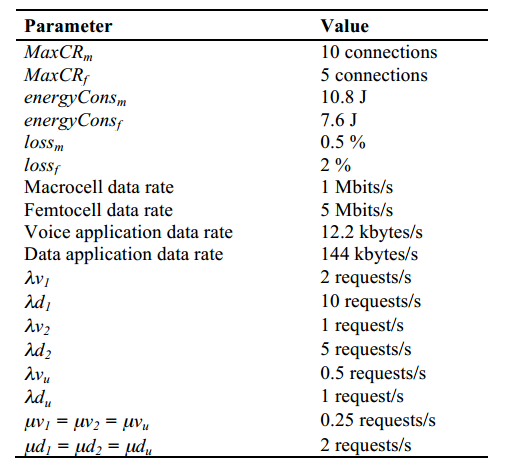
\includegraphics [width=0.45\textwidth]{./Figures/val_1}
  \end{figure} 
    \item \scriptsize Em cada cenário é analisado somente uma variável de saída.
    \item \scriptsize Durante a avaliação a variável analisada tem seu custo definido com valor 1 e as demais com valor 0.
  \end{itemize}    
\end{frame}

\begin{frame}{Descrição dos cenários}
  \begin{block}{\footnotesize Cenário 1. (SCEN1)}
    \begin{itemize}
      \item \footnotesize \alert{Objetivo:} Minimizar  o custo de consumo de energia. Método similar ao implementado pelas operadoras de comunicação atuais utilizando a rede com melhor potencia de sinal.
    \end{itemize}
  \end{block}
  
  \begin{block}{\footnotesize Cenário 2. (SCEN2)}
    \begin{itemize}
      \item \footnotesize \alert{Objetivo:} Maximizar o uso da rede baseado no melhor desempenho na taxa de transferência como critério.
    \end{itemize}
  \end{block}

  \begin{block}{\footnotesize Cenário 3. (SCEN3)}
    \begin{itemize}
      \item \footnotesize \alert{Objetivo}: Maximizar o uso da rede com melhor qualidade de serviço oferecida ao usuário , estabilidade de sinal.
    \end{itemize}
  \end{block}
\end{frame}

\begin{frame}{Descrição dos cenários}
  \begin{block}{Tabela exibindo os parâmetros dos três cenários:}
    \begin{itemize}
      \item \scriptsize Custo de energia.
      \item \scriptsize Custo da perda de voz.
      \item \scriptsize Custo da perda de dados.
      \item \scriptsize Custo taxa de transf. voz.
      \item \scriptsize Custo taxa de transf. dados.
    \end{itemize}    
  \end{block}
   
    \begin{figure}
      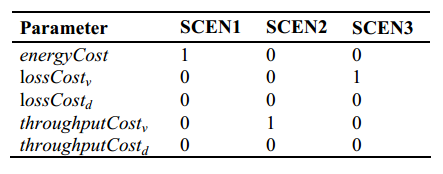
\includegraphics [width=0.65\textwidth]{./Figures/val_2}
    \end{figure}
\end{frame}

\begin{frame}{Resultado da avaliação}
  \begin{itemize}
    \item Resultados obtidos para os cenários avaliados, analisando as seguintes variáveis conforme a tabela:
  \end{itemize}
  \begin{figure}
    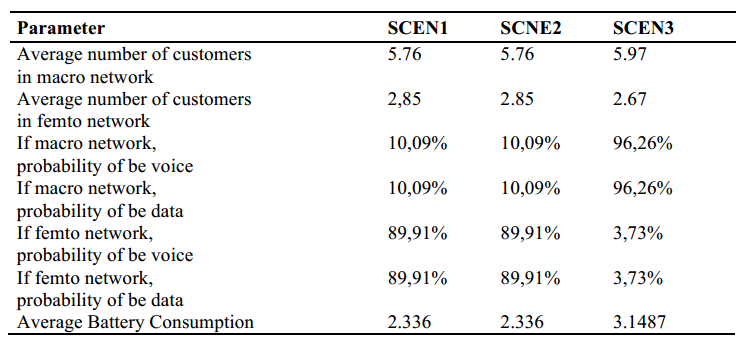
\includegraphics [width=0.75\textwidth]{./Figures/val_3}
  \end{figure}
\end{frame}

\begin{frame}
  \begin{block}{Resultado da avaliação}
    \begin{itemize}
      \item \footnotesize Nos cenários SCEN1 e SCEN2 conforme a tabela, os resultados são equivalentes, devido a rede femtocell ter os atributos preferenciais como potência do sinal e taxa de transferência.
      \newline
      \item \footnotesize Sendo \alert{89,1\%} das requisições atendidas pela rede femto e \alert{10,9\%} ser atendido pela rede macro.
      \newline
      \item \footnotesize Já em SCEN3 a rede macroCell atingiu \alert{96,26\%} das requisições devido ao baixo percentual de perda de \alert{0,5\%} enquanto da rede femto é de \alert{2\%}.
      \newline
      \item \footnotesize O custo de energia em SCEN3 sofreu alteração devido a distancia do transmissor e a rede macroCell ser a preferencial para as conexões já que é avaliado a qualidade do serviço, aumentando em \alert{25,79\%} o consumo de energia.
    \end{itemize}
  \end{block}
\end{frame}
